%%%%%%%%%%%%%%%%%%%%%%%%%%%%%%%%%%%%%%%%%%%%%%%%%%%%%%%%%%%%%%%%%%%
%                                                                 %
%                            CHAPTER FIVE                          %
%                                                                 %
%%%%%%%%%%%%%%%%%%%%%%%%%%%%%%%%%%%%%%%%%%%%%%%%%%%%%%%%%%%%%%%%%%%
\chapter{Pilot User Study} \label{sec:pilot}

In the previous chapters, I described in detail the modifications to OASIS and the rationale behind those changes. In order to confirm the validity of this work, I performed a small pilot user study on 6 students aimed at determining the usability and accuracy of this sketching interface compared to the classic interface on OASIS. This chapter will outline and briefly analyze the feedback received from those participating in the study.

\section{Study Conditions and Methods}
%how were they asked (phone, in person)
%under what conditions did they perform the study
%how much did I guide them

%guidelines I tried to follow

Participants participated in one of two scenarios: in person questioning or over the phone. I attempted to keep the experience the same for both types of participants. Those that partook in person had access to a Wacom Intuos CTL490DW digital drawing tablet, and those who participated over the phone did not. Aside from a brief overview of the project itself, all users were guided minimally once logged onto OASIS. However, I was available for guidance throughout the study and answered all questions to the best of my ability. All participants were asked to draw a room of their choice on each of the user interfaces. The first interface, the drag-and-drop interface is the `classic` version of the interface. The second interface is the sketching interface, and emulates sketching with a pencil. Participants were allowed design on the interfaces in any order. Neither interface design proceeded past the design phase, and did not proceed to the 3D model generation. Afterwards, all participants were asked the same series of questions about their experience. 

\section{Questions and Goals}
The following questions were asked to each of 6 participants after each design, and their responses were recorded. The primary goals of this user study are to isolate the positives and negatives from both systems, learn from them, and apply them accordingly to improve OASIS. Since most of the development of this thesis has been done in isolation, it is enlightening to gather feedback on my work. Another goal is to learn more about other users' perceptions of the interface's usability, and if anything is unclear or confusing. Finally, one last goal is find areas of improvement and new features that users desire in such a system.

\subsection{Questions}
\begin{enumerate}
\item Questions per user:
\begin{itemize}
    \item If any, do you have any experience or formal education in architecture or visual arts? If so, which one and how many years?
    \item Do you have experience with modeling software? If so, which ones?
\end{itemize}
\item Questions per user interface, per design:
\begin{itemize}
    \item On a scale of 1 to 5 (5 being the most confident), how confident are you in your accuracy of design? (dimensions, scale, layout) Why is this your score?
    \item If anything, what did you find fun or interesting about this sketching environment?
    \item Describe designs you were unable to create due to system limitations.
    \item Was there anything you did not like about working in this sketching environment?
    \item Were there any parts of the interface that were hard to use or confusing?
\end{itemize}
\item Questions only for the new sketching interface:
\begin{itemize}
    \item Describe your impressions of the system’s effectiveness in interpreting your design.
    \item Rate on scale of 1 to 5 (5 being the highest), the accuracy to which the system displayed your design, based on your intentions. Why is this your score?
\end{itemize}
\end{enumerate}

\section{Responses and Analysis}
The before mentioned process was conducted with group of fellow students of mixed backgrounds. No students that participated had any familiarity with either system, or any formal experience with architecture. Overall, feedback on the sketching interface was mixed. Users appreciated the flexibility and freedom the new interface offered, but still felt it was lacking in possible features. There was a general concensus that a lack of directions or list of available actions made it difficult to use at first. However, most users agreed it was relatively enjoyable to use and showed potential. Below are some direct quotes about the new system offered by the participants:

\begin{itemize}
    \item Positives:
    \begin{itemize}
        \item  "I thought it was pretty cool, I could draw whatever shapes I wanted".
        \item "It's pretty awesome to scribble stuff out."
        \item "After using the new system, I felt more constrained [in the old system] in terms of what I could make. I couldn’t make the furniture whatever size I wanted."
        \item "Overall it’s pretty fun [...] I thought it would be like Microsoft paint but its like a step beyond that."
        \item "It's pretty fun to just draw stuff and scribble it out."
    \end{itemize}
    \item Negatives:
    \begin{itemize}
        \item "The shapes it can recognize are too limited, what about other shapes like circles and triangles?"
        
        \item "Sometimes it wouldn’t recognize a rectangle that I’m pretty sure is a rectangle."
        
        \item "The classifications on furniture and stuff seemed pretty random."
        
        \item "It feels flexible but limited at the same time, I felt like I could draw anything but the system couldn't handle everything."
        
        \item "I was confused at first what it could do and what I could do."
        
    \end{itemize}
\end{itemize}

\begin{figure}[ht]
\centering
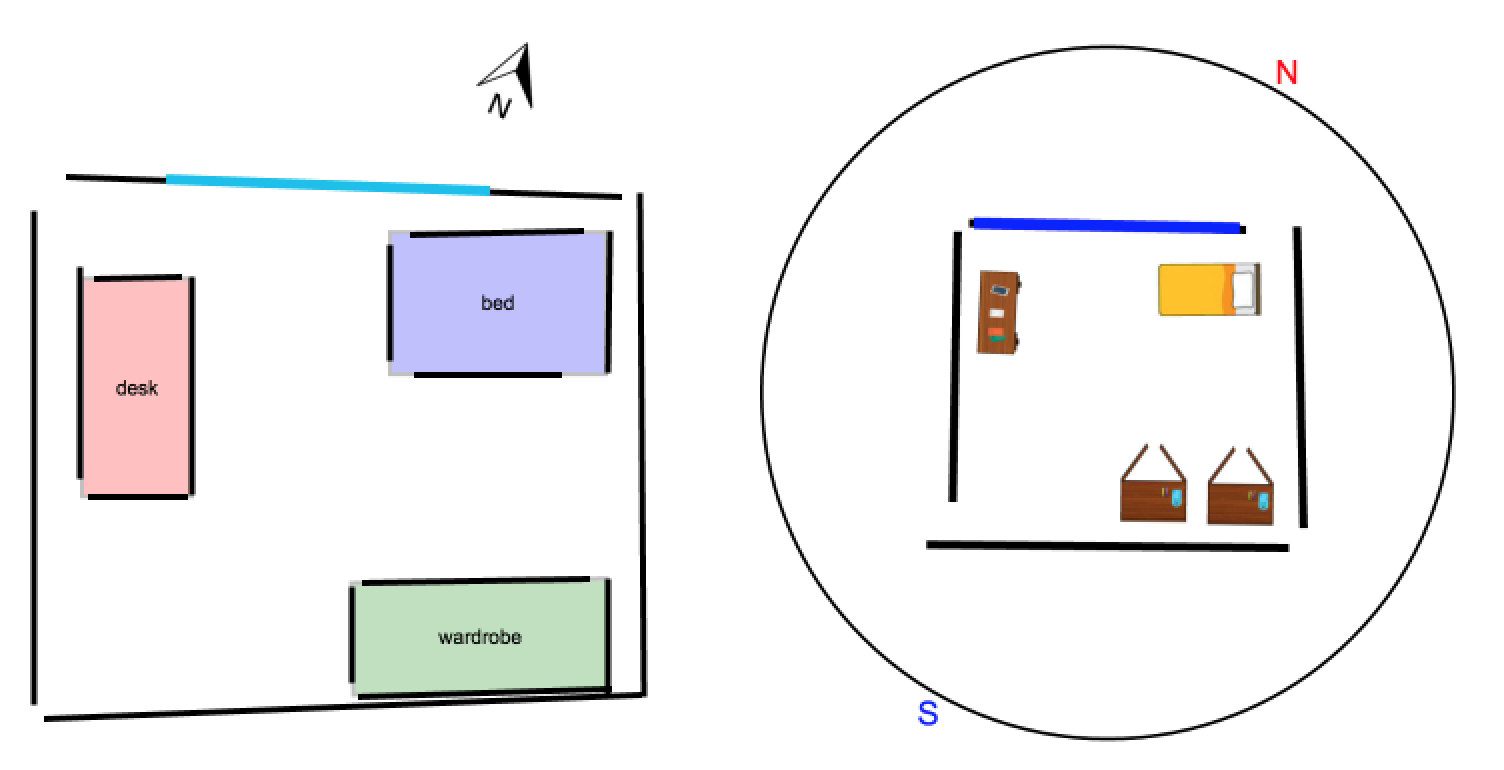
\includegraphics[width=\textwidth]{comparison}
\caption[Comparison of user designed models]{Shown above are two models created by the same user of the same room.}
\label{fig:comparison}
\end{figure}

An overwhelming concern with the new system was its lack of in-system guidance and assistance. Where the classic system had a help menu and instructional video, no similar support was available for the new sketching interface. This caused initial confusion and indecisiveness amongst all participants. However, as the users discovered and learned about its features, most embraced the possibilities it offered.

\begin{figure}[ht]
\centering
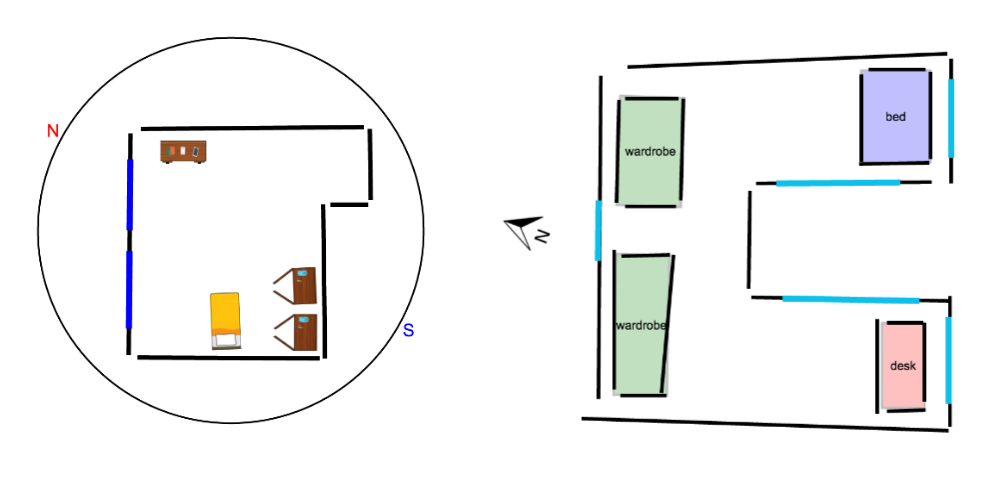
\includegraphics[width=.9\textwidth]{userdrawings}
\caption[Additional user created drawings for the pilot study]{Shown above are two additional models created by users who participated in the study.}
\label{fig:moredrawings}
\end{figure}

Visually, comments were made concerning the lack of images in the new interface. The classic interface overlaid an image of the furniture, clearly indicating what type of furniture it was. The sketching interface had a labels and colors, but the participants found it more visually pleasing to look at images instead of monochromatic blocks. \\

\begin{figure}[ht]
\centering
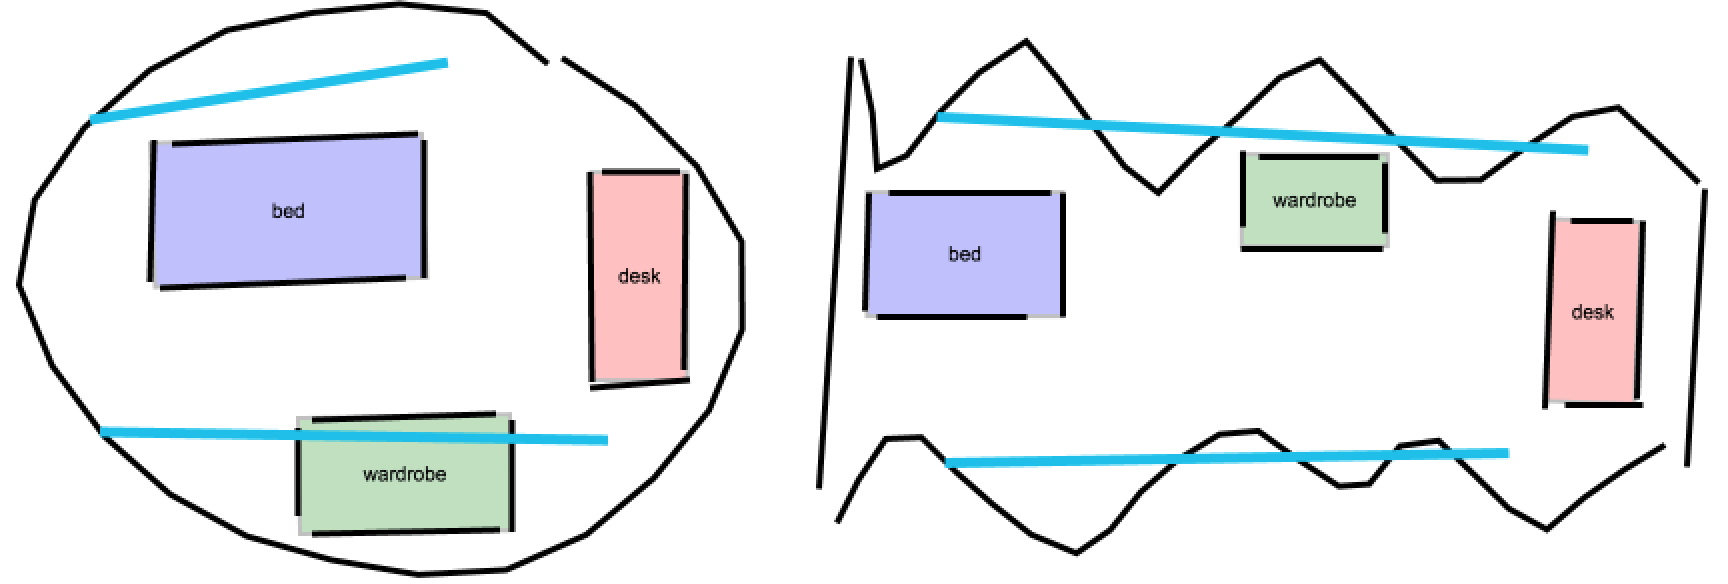
\includegraphics[width=.9\textwidth]{badwindows}
\caption[Examples of windows not snapping correctly]{Shown above are two models where the windows did not snap correctly to the walls they were attached to.}
\label{fig:badwindows}
\end{figure}

The order in which the participants chose to use the interface seemed to have a surprising impact on their feedback. Those that chose the new sketching interface first felt more constrained in their available design choices once they started using the classic interface. The users that chose to use the classic interface first seemed more conservative in their design choices. Typically, the interface that was chosen second received more criticism. Since no users had any prior experience with systems such as this, it made logical sense that the first interface they used became the baseline for their sense of comparison.

There were some types of models I was not prepared for, and most problems stemmed from the lack of flexible windows. Two examples are shown in Figure \ref{fig:badwindows}, the left is a single, curved stoke as the surrounding wall, while the right drew a jagged edge as a whole wall. As explained in chapter 3, the window snapping algorithm uses the line of best fit of the wall it is attempting to attach to. This approach works well for straight lines. However, for strokes similar to an ellipse and highly jagged lines, the result is clearly faulty. I was the primary user of this system during development, and it never occurred to me to even attempt to create a wall for a building that was not straight, let alone attach a window to it. This result only reiterates the importance of user studies. We as developers cannot anticipate the actions of the user, and through studies such as this we can make our systems more robust.

Overall, this pilot study gave a sense of other users' opinions of the system, as well as some welcomed initial feedback. However, in the event of a more detailed user study, there must be a greater attention to detail. If a proper user study is to be conducted, more details about each participant must be recorded. A greater variety of participants is also necessary to gain a broader variety of opinions. Recording details about the usage of the system and each user's actions would allow a more in-depth analysis of the system. This pilot study made some good first steps, but further adjustments must be made for a more comprehensive user study.

\section{Chapter Summary}

This chapter summarizes a brief pilot study performed to determine the effectiveness of this work against the previous user interface of OASIS. Results and feedback were diverse, clearly showing where this work has succeeded and failed. Through the lessons learned in this study, I have identified areas of improvement and possible features for the future. 